%% Screen version %%%%%%%%%%%%%%%%%%%%%%%%%%%%%%%%%%%%%%%%%%%%%%%%%%%%%%%%%%%%%%
\documentclass[xcolor=x11names,compress]{beamer}

% Handout version %%%%%%%%%%%%%%%%%%%%%%%%%%%%%%%%%%%%%%%%%%%%%%%%%%%%%%%%%%%%%%
%\documentclass[xcolor=x11names,compress,handout]{beamer}
%
%\usepackage{pgfpages}
%\pgfpagesuselayout{4 on 1}[a4paper,landscape,border shrink=5mm]

% Ładniejsze tabelki
\usepackage{booktabs}

%% General document %%%%%%%%%%%%%%%%%%%%%%%%%%%%%%%%%%%%%%%%%%%%%%%%%%%%%%%%%%%%
\usepackage{graphicx}
\usepackage[MeX]{polski}

\usepackage[absolute]{textpos}

\usepackage{fancybox}

\usepackage{multicol}


\usepackage[utf8]{inputenc}
\usepackage{tikz}
\usetikzlibrary{decorations.fractals}
%%%%%%%%%%%%%%%%%%%%%%%%%%%%%%%%%%%%%%%%%%%%%%%%%%%%%%%%%%%%%%%%%%%%%%%%%%%%%%%%


%% Beamer Layout %%%%%%%%%%%%%%%%%%%%%%%%%%%%%%%%%%%%%%%%%%%%%%%%%%%%%%%%%%%%%%%
\useoutertheme[subsection=false,shadow,footline=authortitle]{miniframes}
\useinnertheme{default}
\usefonttheme{serif}
\usepackage[T1]{fontenc}
\usepackage{palatino}

\setbeamerfont{title like}{shape=\scshape}
\setbeamerfont{frametitle}{shape=\scshape}

\setbeamercolor*{lower separation line head}{bg=DeepSkyBlue4}
\setbeamercolor*{upper separation line foot}{bg=DeepSkyBlue4}
\setbeamercolor*{normal text}{fg=black,bg=white}
\setbeamercolor*{alerted text}{fg=DeepSkyBlue4}
\setbeamercolor*{example text}{fg=black}
\setbeamercolor*{structure}{fg=DeepSkyBlue4}
\setbeamercolor*{itemize item}{fg=DeepSkyBlue4}

\setbeamercolor*{palette tertiary}{fg=black,bg=black!10}
\setbeamercolor*{palette quaternary}{fg=black,bg=black!10}

\setbeamersize{
  text margin left=1cm,
  text margin right=1cm
}

\newcommand{\code}[1]{\textit{#1}}

\renewcommand{\(}{\begin{columns}}
\renewcommand{\)}{\end{columns}}
\newcommand{\<}[1]{\begin{column}{#1}}
\renewcommand{\>}{\end{column}}

% definicja symboli do tabeli cech
\def\YES{\CIRCLE}        % posiada
\def\HALF{\LEFTcircle}   % częściowo posiada
\def\NO{\Circle}         % nie posiada
\def\NA{$\times$}          % nie dotyczy


%%%%%%%%%%%%%%%%%%%%%%%%%%%%%%%%%%%%%%%%%%%%%%%%%%%%%%%%%%%%%%%%%%%%%%%%%%%%%%%%

\setcounter{tocdepth}{2}

% The following command gets rid of the navigation symbols that you usually
% see at the bottom-right of people's Beamer talks.
%
\setbeamertemplate{navigation symbols}{}

\setbeamercovered{transparent}

\begin{document}

\title{Wykorzystanie informacji z kamery 3D do nawigacji robota mobilnego}
\author{Maciej Stefańczyk}
\institute{\it Wydział Elektroniki i Technik Informacyjnych Politechniki Warszawskiej

\begin{figure}[h!]
\centering
\includegraphics[width=4.4cm]{img/depth_of_field}
\label{fig:p1}
\end{figure}
}

\date{\today}

\AtBeginSection[]
{
  \begin{frame}<beamer>
    \frametitle{Plan prezentacji}
    \begin{multicols}{2}
    \small
    \tableofcontents[currentsection]
    \end{multicols}

  \end{frame}
}

%%%%%%%%%%%%%%%%%%%%%%%%%%%%%%%%%%%%%%%%%%%%%%%%%%%%%%%%%%%%%%%%%%%%%%%%%%%%%%%%
%%%%%%%%%%%%%%%%%%%%%%%%%%%%%%%%%%%%%%%%%%%%%%%%%%%%%%%%%%%%%%%%%%%%%%%%%%%%%%%%

\setbeamercolor{normal text}{bg=black!10}

\begin{frame}[plain]

\titlepage
\end{frame}

\setbeamercolor{normal text}{bg=}

%%%%%%%%%%%%%%%%%%%%%%%%%%%%%%%%%%%%%%%%%%%%%%%%%%%%%%%%%%%%%%%%%%%%%%%%%%%%%%%%
%%%%%%%%%%%%%%%%%%%%%%%%%%%%%%%%%%%%%%%%%%%%%%%%%%%%%%%%%%%%%%%%%%%%%%%%%%%%%%%%
\begin{frame}{Plan prezentacji}
	\frametitle{Plan prezentacji}
	\begin{multicols}{2}
	\small
	\tableofcontents
	\end{multicols}
\end{frame}

%%%%%%%%%%%%%%%%%%%%%%%%%%%%%%%%%%%%%%%%%%%%%%%%%%%%%%%%%%%%%%%%%%%%%%%%%%%%%%%%
%
% Wstęp
%
%%%%%%%%%%%%%%%%%%%%%%%%%%%%%%%%%%%%%%%%%%%%%%%%%%%%%%%%%%%%%%%%%%%%%%%%%%%%%%%%
\section{\vspace{.3cm}\scshape Wstęp}

\begin{frame}{Wstęp}

\alert{Cel pracy}
\begin{itemize}
\item fuzja danych z wielu czujników,
\item trójwymiarowa mapa otoczenia,
\item sprawna nawigacja w dynamicznie zmiennym środowisku.
\end{itemize}

\vspace{.5cm}

\alert{Dotychczasowe rozwiązania}
\begin{itemize}
\item wykorzystanie jedynie częściowej informacji o scenie,
\item powolne skanowanie przestrzeni czujnikami 1D/2D,
\item wykorzystanie drogich czujników 3D.
\end{itemize}

\end{frame}

%%%%%%%%%%%%%%%%%%%%%%%%%%%%%%%%%%%%%%%%%%%%%%%%%%%%%%%%%%%%%%%%%%%%%%%%%%%%%%%%
%
% Źródła obrazu 3D
%
%%%%%%%%%%%%%%%%%%%%%%%%%%%%%%%%%%%%%%%%%%%%%%%%%%%%%%%%%%%%%%%%%%%%%%%%%%%%%%%%
\section{\scshape Źródła obrazu 3D}

%%%%%%%%%%%%%%%%%%%%%%%%%%%%%%%%%%%%%%%%%%%%%%%%%%%%%%%%%%%%%%%%%%%%%%%%%%%%%%%%
%%%%%%%%%%%%%%%%%%%%%%%%%%%%%%%%%%%%%%%%%%%%%%%%%%%%%%%%%%%%%%%%%%%%%%%%%%%%%%%%
\subsection{Stereowizja}

\begin{frame}{Stereowizja: zasada działania}

    \alert{Podstawy teoretyczne}
    \begin{itemize}[<+->]
    \item parametry kamery\\(zewnętrzne i wewnętrzne),
    \item geometria epipolarna.
    \end{itemize}

    \vspace{.5cm}

    \alert{Potok przetwarzania}
    \begin{itemize}[<+->]
    \item akwizycja z kamer,
    \item rektyfikacja obrazu,
    \item detekcja i dopasowanie\\punktów charakterystycznych,
    \item rekonstrukcja współrzędnych\\trójwymiarowych.
    \end{itemize}

\only<1,2>{
\begin{textblock*}{50mm}(70mm,20mm)%
%  \noindent\colorbox[rgb]{0,1,0}{%
    \begin{minipage}[l]{50mm}%

	\begin{figure}[h!]
    \centering
    \includegraphics[width=4.6cm]{../Common/img/camera_intrinsics}
    \end{figure}

    \end{minipage}
%  }%
\end{textblock*}}

\only<2>{
\begin{textblock*}{50mm}(70mm,60mm)%
  %\noindent\colorbox[rgb]{0,1,1}{%
    \begin{minipage}[l]{50mm}%

	\begin{figure}[h!]
    \centering
    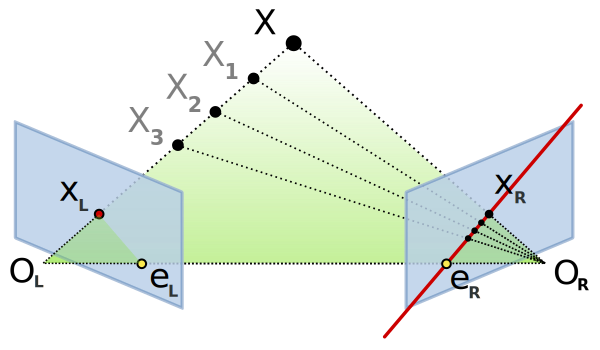
\includegraphics[width=4.6cm]{../Common/img/Epipolar_geometry}
    \end{figure}

    \end{minipage}
  %}%
\end{textblock*}}


\only<3,4,5,6>{
\begin{textblock*}{50mm}(70mm,20mm)%
%  \noindent\colorbox[rgb]{0,1,0}{%
    \begin{minipage}[l]{50mm}%

	\begin{figure}[h!]
    \centering
    \includegraphics[width=4.8cm]{../Common/img/stereo_input}
    \end{figure}

    \end{minipage}
%  }%
\end{textblock*}}

\only<4,5,6>{
\begin{textblock*}{50mm}(70mm,40mm)%
%  \noindent\colorbox[rgb]{0,1,0}{%
    \begin{minipage}[l]{50mm}%

	\begin{figure}[h!]
    \centering
    \includegraphics[width=4.8cm]{../Common/img/stereo_rect}
    \end{figure}

    \end{minipage}
%  }%
\end{textblock*}}

\only<6>{
\begin{textblock*}{50mm}(70mm,60mm)%
%  \noindent\colorbox[rgb]{0,1,0}{%
    \begin{minipage}[l]{50mm}%

	\begin{figure}[h!]
    \centering
    \includegraphics[width=3.0cm]{../Common/img/stereo_depth}
    \end{figure}

    \end{minipage}
%  }%
\end{textblock*}}

\end{frame}





\begin{frame}{Stereowizja: sprzęt}

    \alert{Akwizycja obrazu}
    \begin{itemize}
    \item kamery cyfrowe -- wysoka jakość obrazu, wysoka cena,
    \item kamery analogowe -- jakość obrazu zależy od kart akwizycji,
    \item kamery internetowe -- niska jakość obrazu, niska cena.
    \end{itemize}

    \vspace{.3cm}

    \alert{Problemy mechaniczne}
    \begin{itemize}
    \item stabilne mocowanie kamer.
    \end{itemize}

    \vspace{.3cm}

    \alert{Obliczenia}
    \begin{itemize}
    \item rozwiązania sprzętowe oparte o FPGA,
    \item komputer osobisty.
    \end{itemize}

\end{frame}

\begin{frame}{Stereowizja: właściwości}

    \alert{Szybkość działania}
    \begin{itemize}
    \item proste algorytmy: kilkanaście klatek na sekundę,
    \item złożone, wieloetapowe: do kilkunastu minut na klatkę.
    \end{itemize}

    \vspace{1cm}

    \alert{Pokrycie obszaru widzenia}
    \begin{itemize}
    \item czas rzeczywisty != pełne pokrycie,
    \item łatwo przeoczyć przeszkody.
    \end{itemize}

\end{frame}

\begin{frame}{Stereowizja: rezultaty I}

    \begin{figure}[h!]
    \centering
    \includegraphics[width=11cm]{../Common/img/stereo_2}
    \caption{Obiekty o zróżnicowanej teksturze.}
    \label{fig:stereo_2}
    \end{figure}

\end{frame}


\begin{frame}{Stereowizja: rezultaty II}

    \begin{figure}[h!]
    \centering
    \includegraphics[width=11cm]{../Common/img/stereo_3}
    \caption{Problemy z~dużymi, jednolitymi przeszkodami.}
    \label{fig:stereo_3}
    \end{figure}

\end{frame}

%%%%%%%%%%%%%%%%%%%%%%%%%%%%%%%%%%%%%%%%%%%%%%%%%%%%%%%%%%%%%%%%%%%%%%%%%%%%%%%%
%%%%%%%%%%%%%%%%%%%%%%%%%%%%%%%%%%%%%%%%%%%%%%%%%%%%%%%%%%%%%%%%%%%%%%%%%%%%%%%%
\subsection{Kamery TOF}

\begin{frame}{Kamery TOF: zasada działania}

    \vspace{.5cm}

    \alert{TOF} -- time of flight, czas przelotu wiązki światła.

    \vspace{0.2cm}

    \alert{Działanie}
    \begin{itemize}
    \item emisja błysku światła (podczerwień),
    \item pomiar czasu powrotu wiązki odbitej od obiektów.
    \end{itemize}

    \begin{figure}[h!]
    \centering
    \includegraphics[height=3cm]{../Common/img/tof}
    \caption{Przykład układu mierzącego czas przelotu wiązki światła.}
    \label{fig:tof}
    \end{figure}

\end{frame}



\begin{frame}{Kamery TOF: sprzęt i właściwości}

	\alert{Parametry kamer}
	\begin{itemize}
	\item rozdzielczość głębi do 400x400 pikseli,
	\item szybkość działania od kilkunastu do 100 klatek na sekundę,
	\item przetwarzanie całkowicie sprzętowe.
	\end{itemize}

	\vspace{.7cm}

	\alert{Wady}
	\begin{itemize}
	\item wysoka cena urządzeń,
	\item problemy z interferencją.
	\end{itemize}

\end{frame}

%%%%%%%%%%%%%%%%%%%%%%%%%%%%%%%%%%%%%%%%%%%%%%%%%%%%%%%%%%%%%%%%%%%%%%%%%%%%%%%%
%%%%%%%%%%%%%%%%%%%%%%%%%%%%%%%%%%%%%%%%%%%%%%%%%%%%%%%%%%%%%%%%%%%%%%%%%%%%%%%%
\subsection{\vspace{2cm}Światło strukturalne}

\begin{frame}{Światło strukturalne: zasada działania}

    \vspace{1cm}
    \alert{Potok przetwarzania}
    \begin{itemize}[<+->]
    \item oświetlenie sceny znanym wzorem/sekwencją wzorów,
    \item przyporządkowanie pikseli obrazu do pozycji we wzorcu,
    \item obliczenie pozycji punktów w przestrzeni.
    \end{itemize}

    \begin{figure}[h!]
    \centering
    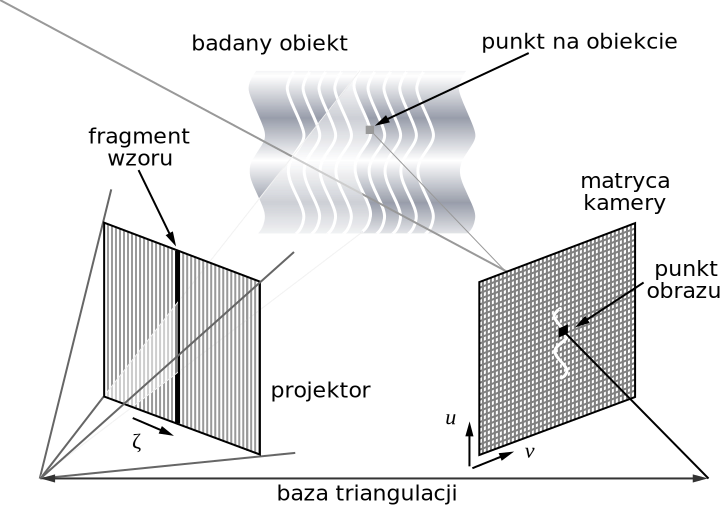
\includegraphics[height=3cm]{../Common/img/struct}
    \caption{Układ pomiarowy wykorzystujący światło strukturalne.}
    \label{fig:struct}
    \end{figure}

\end{frame}

\begin{frame}{Światło strukturalne: właściwości}

    \vspace{.3cm}
    \alert{Wymagania}
    \begin{itemize}
    \item pojedyncza kamera,
    \item projektor.
    \end{itemize}

    \pause
    \vspace{.2cm}

    \alert{Obliczenia}
    \begin{itemize}
    \item sceny statyczne -- wzorce wielowarstwowe,
    \item sceny dynamiczne -- pojedyncze wzorce,
    \item implementacje programowe i sprzętowe.
    \end{itemize}

    \pause
    \vspace{.2cm}

    \alert{Wady}
    \begin{itemize}
    \item słabe wykrywanie wąskich obiektów,
    \item interferencja,
    \item zewnętrzne źródła światła.
    \end{itemize}

\end{frame}

\begin{frame}{Światło strukturalne: przykłady}

    \begin{textblock*}{128mm}(0mm,20mm)%
%  \noindent\colorbox[rgb]{0,1,0}{%
    \begin{minipage}[l]{128mm}%

	\begin{figure}[h!]
    \centering
    \includegraphics[width=10cm]{../Common/img/struct_all}
    \end{figure}

    \end{minipage}
%  }%
    \end{textblock*}

    \begin{textblock*}{50mm}(70mm,57mm)%
%  \noindent\colorbox[rgb]{0,1,0}{%
    \begin{minipage}[l]{50mm}%

	\begin{figure}[h!]
    \centering
    \includegraphics[width=4.5cm]{../Common/img/struct_patterns}
    \end{figure}

    \end{minipage}
%  }%
    \end{textblock*}

    \begin{textblock*}{70mm}(10mm,50mm)%
%  \noindent\colorbox[rgb]{0,1,0}{%
    \begin{minipage}[l]{70mm}%

    \scriptsize
    \alert{Na górze:} Układ pomiarowy, dwa przykładowe obrazy oraz zrekonstruowany model.

    \vspace{2.5cm}

    \alert{Po prawej:} Różne wykorzystywane wzorce.

    \end{minipage}
%  }%
    \end{textblock*}

\end{frame}

%%%%%%%%%%%%%%%%%%%%%%%%%%%%%%%%%%%%%%%%%%%%%%%%%%%%%%%%%%%%%%%%%%%%%%%%%%%%%%%%
%
% Platforma sprzętowa
%
%%%%%%%%%%%%%%%%%%%%%%%%%%%%%%%%%%%%%%%%%%%%%%%%%%%%%%%%%%%%%%%%%%%%%%%%%%%%%%%%
\section{\scshape Platforma sprzętowa}

%%%%%%%%%%%%%%%%%%%%%%%%%%%%%%%%%%%%%%%%%%%%%%%%%%%%%%%%%%%%%%%%%%%%%%%%%%%%%%%%
%%%%%%%%%%%%%%%%%%%%%%%%%%%%%%%%%%%%%%%%%%%%%%%%%%%%%%%%%%%%%%%%%%%%%%%%%%%%%%%%
\subsection{Microsoft Kinect}

\begin{frame}{Kinect: informacje}

    \begin{tabular}{ll}
    \alert{Producent} & Microsoft\\
    \alert{Funkcja} & kontroler gier do Xbox\\
    \alert{Premiera} & 4 listopada 2010r. \\
    \alert{Sprzedano} & ponad 10 mln. szt. (9.03.2011)\\
    \alert{Cena} & ok. 500PLN\\
    \end{tabular}

    \pause
    \vspace{1cm}

    \alert{Sterowniki}
    \begin{itemize}
    \item oficjalnie wspierany jedynie na Xbox,
    \item Microsoft zapowiedział udostępnienie sterowników na Windows,
    \item nieoficjalne sterowniki dla Windows, Linux oraz MacOS.
    \end{itemize}

\end{frame}


\begin{frame}{Kinect: budowa}

    \begin{figure}[h!]
    \centering
    \includegraphics[height=6cm]{../Common/img/kinect_hardware}
    \caption{Microsoft Kinect}
    \end{figure}

\end{frame}


\begin{frame}{Kinect: działanie}

    \begin{itemize}
    \item Detekcja oparta o \alert{światło strukturalne},
    \item implementacja całkowicie sprzętowa.
    \end{itemize}

    \vspace{.6cm}

    \begin{tabular}{ll}
    \alert{Obraz głębi} & 320x240x12bpp\\
    \alert{Obraz RGB} & 640x480x24bpp\\
    \alert{Szybkość} & 30 FPS\\
    \alert{Pole widzenia} & H 57, V 43\\
    \alert{Zakres efektywny} & 1.2m - 3.5m\\
    \alert{Dodatkowe czujniki} & akcelerometr 3-osiowy\\
    \end{tabular}

    \begin{textblock*}{50mm}(76mm,33mm)%
%  \noindent\colorbox[rgb]{0,1,0}{%
    \begin{minipage}[l]{50mm}%

    \begin{figure}[h!]
    \centering
    \includegraphics[width=4.6cm]{../Common/img/kinect_pattern}
    \caption{Wzór wykorzystywany przez Kinect}
    \end{figure}

    \end{minipage}
%  }%
\end{textblock*}

\end{frame}


\begin{frame}{Kinect: rezultaty I}

    \begin{figure}[h!]
    \centering
    \includegraphics[width=11cm]{../Common/img/kinect_2}
    \caption{Obiekty o zróżnicowanej teksturze.}
    \end{figure}

\end{frame}


\begin{frame}{Kinect: rezultaty II}

    \begin{figure}[h!]
    \centering
    \includegraphics[width=11cm]{../Common/img/kinect_3}
    \caption{Obiekty o jednolitej teksturze.}
    \end{figure}

\end{frame}


\begin{frame}{Kinect: porównanie ze stereowizją}

    \begin{figure}[h!]
    \centering
    \includegraphics[width=11cm]{../Common/img/kinect_vs_stereo}
    \caption{Mapy głębi generowane przez algorytm stereowizyjny oraz Kinect.}
    \end{figure}

\end{frame}

%%%%%%%%%%%%%%%%%%%%%%%%%%%%%%%%%%%%%%%%%%%%%%%%%%%%%%%%%%%%%%%%%%%%%%%%%%%%%%%%
%%%%%%%%%%%%%%%%%%%%%%%%%%%%%%%%%%%%%%%%%%%%%%%%%%%%%%%%%%%%%%%%%%%%%%%%%%%%%%%%
\subsection{\vspace{.3cm}Baza mobilna Elektron}

\begin{frame}{Elektron: projekt}

    \vspace{.1cm}

    \alert{Przeznaczenie} -- modułowa baza mobilna przeznaczona do przeprowadzania
    doświadczeń oraz do dydaktyki.

    \vspace{.4cm}

    \alert{Projekt}
    \begin{itemize}
    \item Instytut Automatyki i Informatyki Stosowanej,
    \item Instytut Automatyki i Robotyki,
    \item pierwsza wersja w roku 2006.
    \end{itemize}

    \vspace{.4cm}

    \begin{tabular}{ll}
    \alert{Wymiary bazy} & 500x380x220mm\\
    \alert{Masa bazy} & 20kg\\
    \alert{Nośność} & 100kg\\
    \alert{Napęd} & silniki DC 24V\\
    \alert{Materiał} & aluminium\\
    \end{tabular}

    \begin{textblock*}{50mm}(80mm,40mm)%
%  \noindent\colorbox[rgb]{0,1,0}{%
    \begin{minipage}[l]{50mm}%
    \centering
    \begin{figure}[h!]
    \centering
    \includegraphics[width=4.6cm]{../Common/img/elektron/elektron_kinect}
    %\caption{Robot elektron z~czujnikiem Kinect}
    \end{figure}
    \scriptsize
    \alert{Rysunek:} Robot elektron\\z czujnikiem Kinect oraz LMS100

    \end{minipage}
%  }%
    \end{textblock*}

\end{frame}


\begin{frame}{Elektron: sterowanie}

    \alert{Moduły}
    \begin{itemize}
    \item jasno określone interfejsy,
    \item wzajemna niezależność,
    \item możliwość łatwej wymiany.
    \end{itemize}

    \vspace{.4cm}
    \pause

    \alert{Komputer sterujący}
    \begin{itemize}
    \item pierwotnie PC-104 (PIII-900),
    \item obecnie netbook EeePC (Atom 1.6).
    \end{itemize}

    \vspace{.4cm}
    \pause

    \alert{Komunikacja}
    \begin{itemize}
    \item wewnętrzna: RS232, RS485, ethernet,
    \item zewnętrzna: ethernet, bluetooth.
    \end{itemize}

\end{frame}


\begin{frame}{Elektron: moduły}

    \alert{Sterujące}
    \begin{itemize}
    \item sterownik zasilania (ładowarka, kontrola stanu akumulatorów),
    \item sterownik silników (wzmacniacz mocy, odometria).
    \end{itemize}

    \vspace{.4cm}
    \pause

    \alert{Pomiarowe}
    \begin{itemize}
    \item grupa czujników IR,
    \item lidary SICK (LMS100, LMS200),
    \item jednostka inercyjna (pozycja).
    \end{itemize}

    \vspace{.4cm}
    \pause

    \alert{Wykonawcze}
    \begin{itemize}
    \item lekki manipulator.
    \end{itemize}

\end{frame}

%%%%%%%%%%%%%%%%%%%%%%%%%%%%%%%%%%%%%%%%%%%%%%%%%%%%%%%%%%%%%%%%%%%%%%%%%%%%%%%%
%
% Algorytmy
%
%%%%%%%%%%%%%%%%%%%%%%%%%%%%%%%%%%%%%%%%%%%%%%%%%%%%%%%%%%%%%%%%%%%%%%%%%%%%%%%%
\section{\scshape Platforma programowa}

%%%%%%%%%%%%%%%%%%%%%%%%%%%%%%%%%%%%%%%%%%%%%%%%%%%%%%%%%%%%%%%%%%%%%%%%%%%%%%%%
%%%%%%%%%%%%%%%%%%%%%%%%%%%%%%%%%%%%%%%%%%%%%%%%%%%%%%%%%%%%%%%%%%%%%%%%%%%%%%%%
\subsection{\vspace{.3cm}ROS}

\begin{frame}{ROS: Robot Operating System}

    \alert{System operacyjny dla robotów}
    \begin{itemize}
    \item sterowanie,
    \item symulacja,
    \item wizualizacja.
    \end{itemize}

    \vspace{.5cm}

    \alert{Języki} -- C++, Python, Java, Lisp, Octave

    \vspace{.5cm}

    \alert{Architektura}
    \begin{itemize}
    \item każdy algorytm/sterownik jako osobny proces,
    \item przezroczysta komunikacja międzyprocesowa,
    \item łatwe rozproszenie na kilka maszyn,
    \item dużo narzędzi pomocniczych.
    \end{itemize}

\end{frame}



\begin{frame}{ROS: platformy}


    \vspace{.4cm}

    \alert{Systemy operacyjne}
    \begin{itemize}
    \item pełne wsparcie: Ubuntu,
    \item częściowe wsparcie: OS X, Arch, Fedora, Gentoo, OpenSUSE, Slackware, Debian,
    \item eksperymentalne: Windows, FreeBSD.
    \end{itemize}

    \vspace{.4cm}

    \alert{Roboty}
    \begin{itemize}
    \item AscTec Pelican/Hummingbird, Care-O-bot, Erratic, Lego NXT, PR2
    \end{itemize}

    \begin{figure}[h!]
    \centering
    \includegraphics[width=10.8cm]{../Common/ros/robots}
    \end{figure}

\end{frame}


\begin{frame}{ROS: wykorzystanie}

    \alert{Sterowniki dla Elektrona}
    \begin{itemize}
    \item sterowanie silnikami,
    \item odczyty z lasera i Kinecta,
    \item odczyty z pary stereowizyjnej.
    \end{itemize}

    \vspace{.4cm}

    \alert{Podział zadań}
    \begin{itemize}
    \item komputer na robocie: proste omijanie przeszkód,
    \item komputer stacjonarny: budowa pełnej mapy 3D i globalne planowanie trasy.
    \end{itemize}


\end{frame}

%%%%%%%%%%%%%%%%%%%%%%%%%%%%%%%%%%%%%%%%%%%%%%%%%%%%%%%%%%%%%%%%%%%%%%%%%%%%%%%%
%
% Podsumowanie
%
%%%%%%%%%%%%%%%%%%%%%%%%%%%%%%%%%%%%%%%%%%%%%%%%%%%%%%%%%%%%%%%%%%%%%%%%%%%%%%%%
\section{\scshape Podsumowanie}

%%%%%%%%%%%%%%%%%%%%%%%%%%%%%%%%%%%%%%%%%%%%%%%%%%%%%%%%%%%%%%%%%%%%%%%%%%%%%%%%
%%%%%%%%%%%%%%%%%%%%%%%%%%%%%%%%%%%%%%%%%%%%%%%%%%%%%%%%%%%%%%%%%%%%%%%%%%%%%%%%
\subsection{Dotychczasowe osiągnięcia}

\begin{frame}{Dotychczasowe osiągnięcia}

    \alert{Sprzętowe}
    \begin{itemize}
    \item modernizacja elektroniki robota Elektron,
    \item interfejs łączący Kinect z komputerem PC.
    \end{itemize}

    \vspace{.4cm}
    \pause

    \alert{Programowe}
    \begin{itemize}
    \item sterowniki do Elektrona dla systemu ROS,
    \item symulacja odczytu laserowego na Kinect.
    \end{itemize}

\end{frame}

%%%%%%%%%%%%%%%%%%%%%%%%%%%%%%%%%%%%%%%%%%%%%%%%%%%%%%%%%%%%%%%%%%%%%%%%%%%%%%%%
%%%%%%%%%%%%%%%%%%%%%%%%%%%%%%%%%%%%%%%%%%%%%%%%%%%%%%%%%%%%%%%%%%%%%%%%%%%%%%%%
\subsection{Perspektywy zastosowania}

\begin{frame}{Perspektywy zastosowania}

    \alert{Przemysł}
    \begin{itemize}
    \item nawigacja w dynamicznie zmieniających się środowiskach,
    \item autonomiczne tworzenie trójwymiarowych map wnętrz,
    \item roboty usługowe w laboratoriach.
    \end{itemize}

    \vspace{.4cm}
    \pause

    \alert{Edukacja}
    \begin{itemize}
    \item badania algorytmów sterowania i omijania przeszkód,
    \item prowadzenie zajęć z robotyki (m.in. EMARO),
    \item udział w zawodach robotycznych.
    \end{itemize}

\end{frame}

%%%%%%%%%%%%%%%%%%%%%%%%%%%%%%%%%%%%%%%%%%%%%%%%%%%%%%%%%%%%%%%%%%%%%%%%%%%%%%%%
%%%%%%%%%%%%%%%%%%%%%%%%%%%%%%%%%%%%%%%%%%%%%%%%%%%%%%%%%%%%%%%%%%%%%%%%%%%%%%%%

\subsection*{}
\begin{frame}{}

\it
\Large{Dziękuję za uwagę.}

\begin{figure}[h!]
\centering
\includegraphics[width=3cm]{img/qmark}
\end{figure}

\hfill\Large{Pytania?}

\end{frame}





%%%%%%%%%%%%%%%%%%%%%%%%%%%%%%%%%%%%%%%%%%%%%%%%%%%%%%%%%%%%%%%%%%%%%%%%%%%%%%%%
%%%%%%%%%%%%%%%%%%%%%%%%%%%%%%%%%%%%%%%%%%%%%%%%%%%%%%%%%%%%%%%%%%%%%%%%%%%%%%%%

\end{document}
